%----------------------------------------------------------------------------------------
%	PREAMBUŁA: PAKIETY I KONFIGURACJA DOKUMENTU
%----------------------------------------------------------------------------------------

\documentclass[11pt,a4paper]{report}   % klasa dokumentu i rozmiar czcionki
\usepackage[margin=1in, paperwidth=8.5in, paperheight=11in]{geometry}   % określa wielkość marginesów
\usepackage[utf8]{inputenc}             % kodowanie dokumentu
\usepackage[T1]{fontenc}                % kodowanie czcionki
\usepackage{polski}                     % polski pakiet językowy
\usepackage{lmodern}                    % czcionka Latex Modern zamiast Computer Modern
\usepackage{parskip}                    % usuwa efekty parskip w ToC
\usepackage{indentfirst}                % automatyczne wcięcia pierwszego akapitu
\usepackage{fancyhdr}					% nagłówek i stopka
\usepackage{lastpage}					% potrzebny fancyhdr do numerowania
\usepackage{extramarks}					% potrzebny fancyhdr
\usepackage{booktabs}					% do tabel
\usepackage{multirow}					% do łączenia wierszy w tabeli
\usepackage{multicol}					% do łączenia kolumn w tabeli
\usepackage{graphicx}					% załączanie obrazów
\usepackage{caption}					% zarządzanie podpisami pod floatami
\usepackage{color}						% zmiana koloru czcionki i tła
\usepackage{placeins}		            % zarządzanie floatami
\usepackage{pdflscape}                  % poziome obracanie stron
\usepackage{enumerate}					% typy wyliczeniowe
\usepackage{listings}					% dodawanie plików źródłowych
\usepackage{amsmath}					% wzory matematyczne
\usepackage{amssymb}                    % rozszerzenie amsmath
\usepackage{relsize}					% zmiana wielkości wzorów matematycznych
\usepackage{gensymb}                    % znaki specjalne
\usepackage{hyperref} 					% do linkowania cytatów, floatów
\usepackage{url}                        % generowanie linków ze znakami specjalnymi
\usepackage{tikz}                       % modelowanie wykresów
\usepackage{longtable}                  % rozkładanie tabel na kilka stron

%----------------------------------------------------------------------------------------
%	PREAMBUŁA: DEFINICJE KOMEND
%----------------------------------------------------------------------------------------

\title{Analiza stopnia złośliwości komórek nowotworowych wykorzystująca sieci neuronowe.}
\author{Łukasz Matysiak \\ Kamil Machnicki}
\newcommand{\Class}{Zastosowania informatyki w medycynie}
\newcommand{\Type}{Sprawozdanie}
\newcommand{\ClassDay}{Czwartek}
\newcommand{\ClassTime}{11:15}
\newcommand{\ClassInstructor}{Dr inż. Bartosz Krawczyk}
\newcommand{\University}{Politechnika Wrocławska}
\newcommand{\Department}{Wydział Elektroniki}
\newcommand{\Faculty}{Informatyka}

%----------------------------------------------------------------------------------------
%	PREAMBUŁA: INNE USTAWIENIA
%----------------------------------------------------------------------------------------

\setlength{\parindent}{12pt} % szerokość wcięć w paragrafach
\setlength{\parskip}{1,0em} % odstępy między paragrafami
%\renewcommand{\baselinestretch}{1.20} % wielkość odstępu między wierszami
\renewcommand\headrulewidth{0pt} % wielkość linii nagłówka
\renewcommand\footrulewidth{0pt} % wielkość linii stopki

\usetikzlibrary{calc} % modelowanie wykresów

%----------------------------------------------------------------------------------------
%	PREAMBUŁA: USTAWIENIA NAGŁÓWKA I STOPKI
%----------------------------------------------------------------------------------------

% zastosowanie fancyhdr do stron typu plain
\fancypagestyle{plain}{}
% styl strony stosujący fancyhdr
\pagestyle{fancy}
    % górny-lewy
\lhead{} %{Zarządzanie flotą komputerów i urządzeń mobilnych}
    % górny-środkowy
\chead{} %{\Class\ (\ClassInstructor\ \ClassDay \ClassTime)}
    % górny-prawy
\rhead{} %{\Class\ }
    % dolny-lewy
\lfoot{} %{\firstxmark}
    % dolny-środkowy
\cfoot{Strona\ \thepage\ z\ \protect\pageref{LastPage}}
    % dolny-prawy
\rfoot{} %{\lastxmark}

%----------------------------------------------------------------------------------------
%	STRONA TYTUŁOWA
%----------------------------------------------------------------------------------------

\makeatletter
\renewcommand{\maketitle}{
\begin{titlepage}
    \begin{center}
        
        \huge\textsc{{\University}}\\
        \Large\textsc{{\Department}}\\
        \Large\textsc{{\Faculty}}\par
        
        \vspace*{2cm}
        \LARGE\textsc{\Class}\par
        
        \vspace{20mm}
        \Huge\textbf{\@title}\par
        
        \vspace{3cm}
		\large\textit{Autorzy:}\\ 
        \Large\textbf{\@author}\par 
        
        \vspace {10mm}
        \large\textit{Prowadzący:}\\
        \large\textbf{\ClassInstructor}\par
        \large\textit{Termin zajęć:}\\
        \large\textbf{\ClassDay, godz. \ClassTime}\par

        \vspace{2cm}
		\small Wrocław \\
        \small \@date \\
		
    \end{center}
\end{titlepage}
}
\makeatother

%----------------------------------------------------------------------------------------
%	DOKUMENT
%----------------------------------------------------------------------------------------

\begin{document}

\maketitle
\tableofcontents
\newpage

\chapter{Wstęp}

\section{Cele i założenia projektowe}

\section{Wstęp teoretyczny}

\chapter{Aplikacja}

\section{Wykorzystane technologie}

Aplikacja implementująca sieci neuronowe na potrzeby realizacji tematu oraz wykonująca badania, zrealizowana została przy wykorzystaniu języka \texttt{Python} w wersji \texttt{3.5}.

Głównym modułem, na którym oparto implementację, był \texttt{scikit-learn}. Wykorzystano go przede wszystkim do zbudowania sieci neuronowej uczoną metodą wstecznej propagacji błędu, a także skorzystano z wielu udostępnionych tam rozwiązań, jak na przykład walidacja krzyżowa i selekcja cech. Użyto modułu w wersji deweloperskiej \texttt{0.18.dev0}\footnote{http://scikit-learn.org/dev/documentation.html}, gdyż dopiero od tej wersji można tam korzystać z sieci neuronowych.

Jako implementację drugiego badanego algorytmu - \textit{Extreme Learning Machines}, posłużył moduł \texttt{Python-ELM}\footnote{https://github.com/dclambert/Python-ELM}. Wyznaczony on był na oficjalnej stronie \textit{ELM}\footnote{http://www.ntu.edu.sg/home/egbhuang/elm\_codes.html} jako jedna z bazowych implementacji tegoż algorytmu. Udostępniony kod nie był, niestety, przystosowany do działania pod wersją \textit{Pythona 3}, na potrzeby projektu przerobiono więc kod tak, aby dało się go używać.

Wszystkie wykorzystane moduły i ich przeznaczenie widnieją na poniższej tabeli:

\begin{table}[h!]
    \centering
    \caption{Wykorzystane moduły.}
    \begin{tabular}{p{3cm}p{2cm}p{11cm}}
        \toprule
        \textbf{Nazwa} & \textbf{Wersja} & \textbf{Opis} \\
        \midrule
        \texttt{scikit-learn} & 0.18 & sieć neuronowa uczona metodą wstecznej propagacji błędu, selekcja cech, walidacja krzyżowa, macierz błędu. \\
        \texttt{Python-ELM} & 0.3 & \textit{Extreme Learning Machines}. \\
        \texttt{numpy} & 1.11.0 & Obliczenia numeryczne. \\
        \texttt{matplotlib} & 1.5.1 & Tworzenie wykresów. \\
        \bottomrule
    \end{tabular}
\end{table}

\newpage

\section{Opis implementacji}

Na aplikację skłąda się kilka modułów:

\begin{itemize}
    \item \texttt{main.py} - główny moduł uruchamiający badania.
    \item \texttt{algorithms.py} - uruchamia oba algorytmy.
    \item \texttt{dataset.py} - importuje dane z pliku CSV.
    \item \texttt{grapher.py} - tworzy wykresy z wyników badań.
    \item \texttt{helper.py} - zawiera klasy pomocnicze do przechowywania danych.
    \item \texttt{consts.py} - zawiera ustawienia badań i parametry dla algorytmów.
\end{itemize}

Po uruchomieniu badania przez moduł \texttt{main.py}, w module \texttt{algorithms.py} odbywa się wykonywanie owych badań. Najpierw, na zbiorze zawierającym dane uczące \texttt{X} oraz tablicę wyników \texttt{y} wykonywana jest 10-krotna walidacja krzyżowa przy pomocy \texttt{StratifiedKFold} z modułu \texttt{sklearn.model\_selection}, w wyniku której otrzymywane są indeksy elementów podzielonych na dwa podzbiory - zbiór uczący i testowy:

\begin{verbatim}
 StratifiedKFold(n_folds=n_folds).split(X, y):
\end{verbatim}

W tym momencie następuje też iteracja przez wszystkie wyniki walidacji, gdzie w każdej iteracji odbywa się selekcja \texttt{n}-cech, gdzie \texttt{n} to liczba cech, dla której aktualnie wykonywane są badania:

\begin{verbatim}
 SelectKBest(k=k_best_features).fit(X, y).get_support(indices=True)
\end{verbatim}

Na tak wyselekcjonowanych cechach odbywa się uruchomienie dwóch algorytmów - uczonego metodą wstecznej propagacji błędu (algorytm \textit{BP}) oraz jego szybka wersja losowa \textit{Extreme Learning Machines} (algorytm \textit{ELM}). Najpierw tworzona jest instancja klasyfikatora algorytmu \textit{BP} (opis parametrów użytych do badania znajduje się w rozdziale o badaniach), następnie odbywa się jego uczenie przekazując do funkcji \texttt{fit} zbiór uczący. Na końcu dokonywane jest mierzenie testowanie algorytmu przekazując do funkcji \texttt{score} zbiór testowy.

\begin{verbatim}
 clf = MLPClassifier(...)
 clf.fit(X_train, y_train)
 score = clf.score(X_test, y_test)
\end{verbatim}

Dla algorytmu \texttt{ELM} procedura wygląda bardzo podobnie:

\begin{verbatim}
 elmc = ELMClassifier(...)
 elmc.fit(X_train, y_train)
 score = elmc.score(X_test, y_test)
\end{verbatim}

\newpage

Na końcu dla każdego algorytmu wyliczana jest macierz pomyłek, korzystając z \texttt{confusion\_matrix} z modułu \texttt{sklearn.metrics}.

\begin{verbatim}
conf_matrix = confusion_matrix(y_test, clf.predict(X_test))
conf_matrix = confusion_matrix(y_test, elmc.predict(X_test))
\end{verbatim}

\section{Wdrożenie}

W celu przygotowania aplikacji do działania, należy mając zainstalowaną wersję \texttt{Pythona 3.5} dodać katalog projektu do zmiennej środowiskowej \texttt{PYTHONPATH}. Aby tego dokonać, w katalogu projektu trzeba uruchomić komendę:

\begin{verbatim}
$ export PYTHONPATH="${PYTHONPATH}:${PWD}"
\end{verbatim}

Kolejnym krokiem jest uruchomienie skryptu instalacyjnego \texttt{install.sh}, który to zainstaluje wymagane pakiety z pliku \texttt{requirements.txt} oraz pobierze poprawiony moduł \texttt{Python-ELM} do katalogu \texttt{modules}:

\begin{verbatim}
./install.sh
\end{verbatim}

Teraz można uruchomić aplikację poprzez wywołanie skryptu głównego \texttt{main.py}:

\begin{verbatim}
python3 main.py
\end{verbatim}

Działanie aplikacji powinno się zakończyć wygenerowanymi wykresami.
\chapter{Badania}

\section{Przeprowadzone badania}

Zgodnie z założeniami, badania przeprowadzono dla 5 różnych liczb neuronów w warstwie ukrytej: \textbf{5, 10, 20, 40, 60}.

Badania rozpoczynają się od iteracji przez wybrane liczby neuronów w warstwie ukrytej. W każdej iteracji uruchamiane są testy dla różnych liczb cech, począwszy od 1 a skończywszy na maksymalnej liczbie cech w zbiorze testowym, w tym wypadku 32. W tym momencie następuje n-krotne wykonanie uczenia i klasyfikacji, a z n-próbek wyciągane są wartości skrajne min-max, liczona jest średnia oraz odchylenie standardowe. Uzyskane w ten sposób wartości służą w późniejszym etapie do odpowiedniego zobrazowania wyników na wykresach. Na potrzeby badań uznano, że 5 powtórzeń będzie wystarczające.

Oba algorytmy uruchamiano z różnymi wartościami stałych parametrów. Oto lista niezmiennych parametrów z jakimi uruchamiano algorytm \texttt{BP}:

\begin{table}[h!]
    \centering
    \caption{Parametry algorytmu \texttt{BP}.}
    \begin{tabular}{p{3cm}p{2cm}p{11cm}}
        \toprule
        \textbf{Parametr} & \textbf{Wartość} & \textbf{Opis} \\
        \midrule
        \texttt{algorithm} & \texttt{sgd} & Algorytm działania (\textit{stochastic gradient descent}). \\
        \texttt{max\_iter} & \texttt{10000} & Maksymalna liczba iteracji. \\
        \texttt{alpha} & \texttt{1e-6} & Parametr regularyzacji L2. \\
        \texttt{learning\_rate} & \texttt{constant} & Tempo uczenia. \\
        \texttt{activation} & \texttt{logistic} & Funkcja aktywacji warstwy ukrytej. \\
        \texttt{random\_state} & \texttt{None} & Ziarno dla generatora liczb losowych. \\
        \bottomrule
    \end{tabular}
\end{table}

Dla algorytmu \texttt{ELM} powyższe parametry były takie same, bądź nie trzeba było ich wprowadzać, z jedną różnicą, gdzie jako funkcji aktywacji użyto funkcję \texttt{multiquadric}.

\newpage

\section{Porównanie algorytmów}

Dla 5 neuronów w warstwie ukrytej zauważyć można, że oba algorytmy osgiągneły prawie takie same wyniki oscylujące w okolicy 76\%, niezależne od liczby wyselekcjonowanych cech.

Również czasy uczenia okazały się bardzo podobne. Wystąpiły tutaj jednakże większe fluktuacje, spowodowane przede wszystkim niedokładnością w mierzeniu bardzo małych czasów (rzędu 0.5 milisekundy) oraz dużym odchyleniem standardowym sygnalizowanym na wykresie przez słupki błędu.

Największą różnicę zauważyć jednak można w czasach uczenia się, gdzie algorytm \texttt{ELM} osiągnął o wiele lepsze czasy rzędu 2 milisekund od algorytmu \texttt{BP}, którego średni czas oscylował w okolicy 130 milisekund. Zauważyć zatem można wyraźnie, że algorytm \texttt{ELM} jest średnio 65 razy szybszy od algorytmu \texttt{BP}.

\begin{figure}[h!]
	\centering
	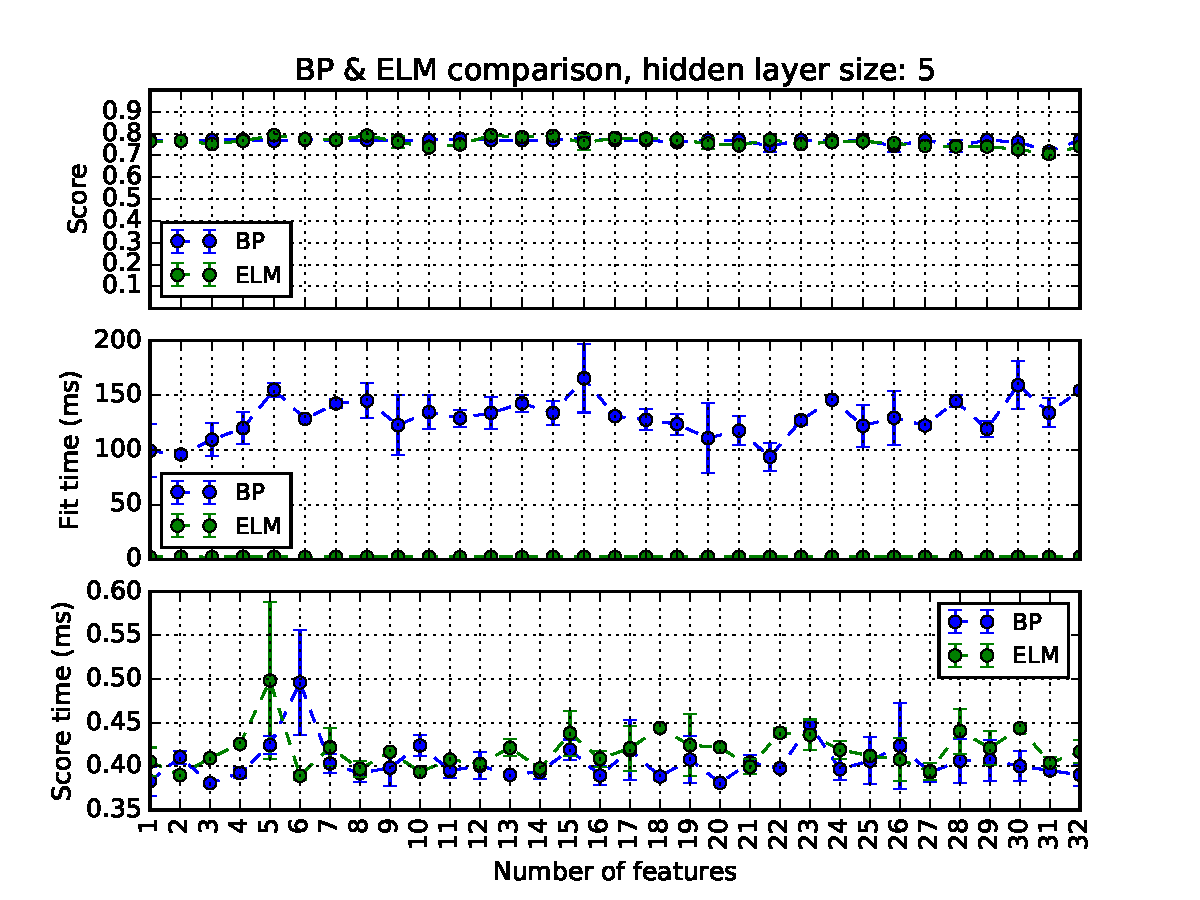
\includegraphics[width=1.0\linewidth]{img/bp_elm_5.pdf}
	\label{Rysunek}
	\caption{5 neuronów w warstwie ukrytej - porównanie obu algorytmów}
\end{figure}

\newpage

Dla 10 neuronów w warstwie ukrytej zachodzą te same zależności. Widoczny jest jednak nieznaczny wzrost czasu uczenia dla algorytmu \texttt{BP} do około 250 milisekund w okolicy 10-14 wyselekcjonowanych cech. Algorytm \texttt{ELM} pozostaje bez zmian.

\begin{figure}[h!]
	\centering
	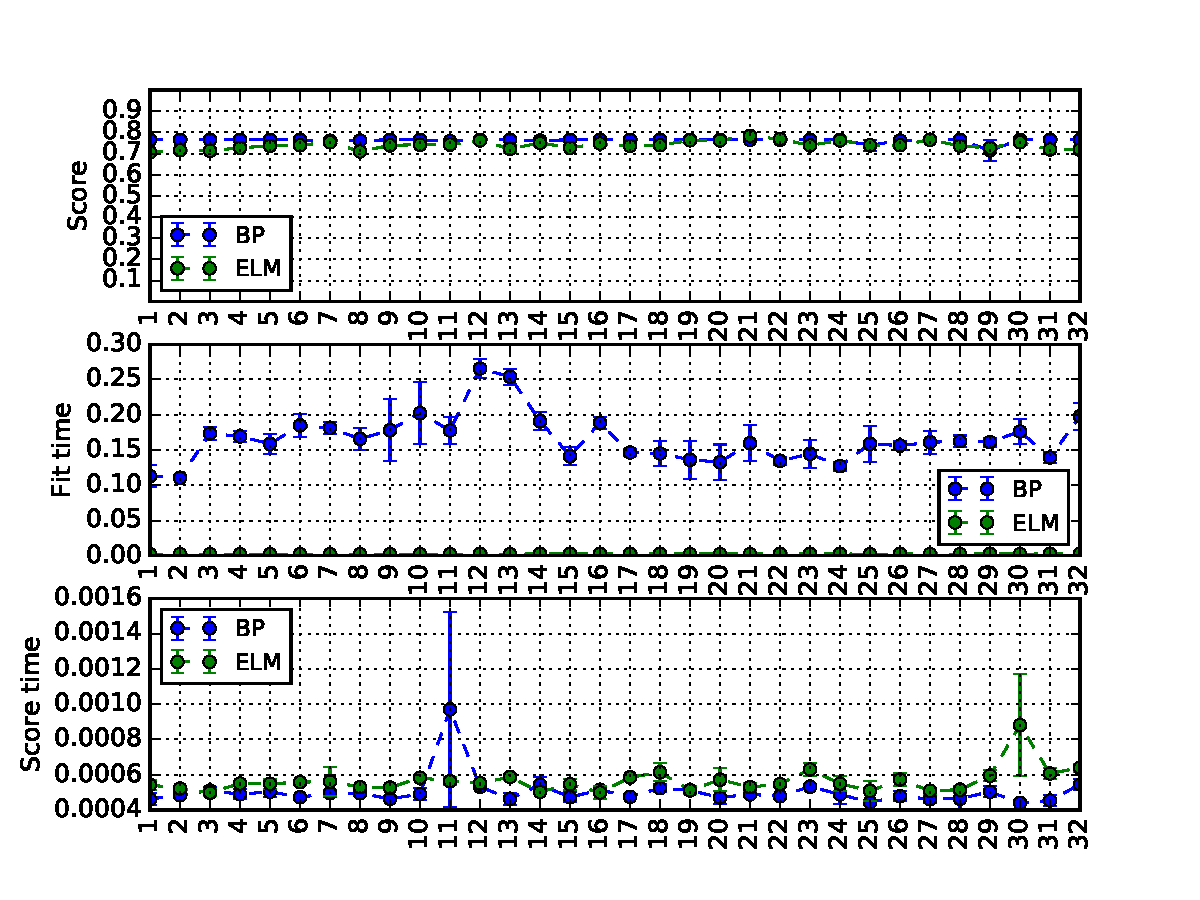
\includegraphics[width=1.0\linewidth]{img/bp_elm_10.pdf}
	\label{Rysunek}
	\caption{10 neuronów w warstwie ukrytej - porównanie obu algorytmów}
\end{figure}

\newpage

Dla 20 neuronów w warstwie ukrytej zdecydowanie zauważyć już można tendencję w czasie uczenia algorytmu \texttt{BP}, gdzie do około 7 wyselekcjonowanych cech czas znacząco wzrasta, później do około 16 sech pozostaje względnie stały, następnie maleje i od 22 cech utrzymuje się już na sałym, niskim poziomie rzędu 100 milisekund. Wytłumaczyć tę zależność można zjawiskiem przeuczenia, gdzie algorytm osiągnął lokalne minima, a następnie je wykorzystywał przy kolejnych uczeniach.

\begin{figure}[h!]
	\centering
	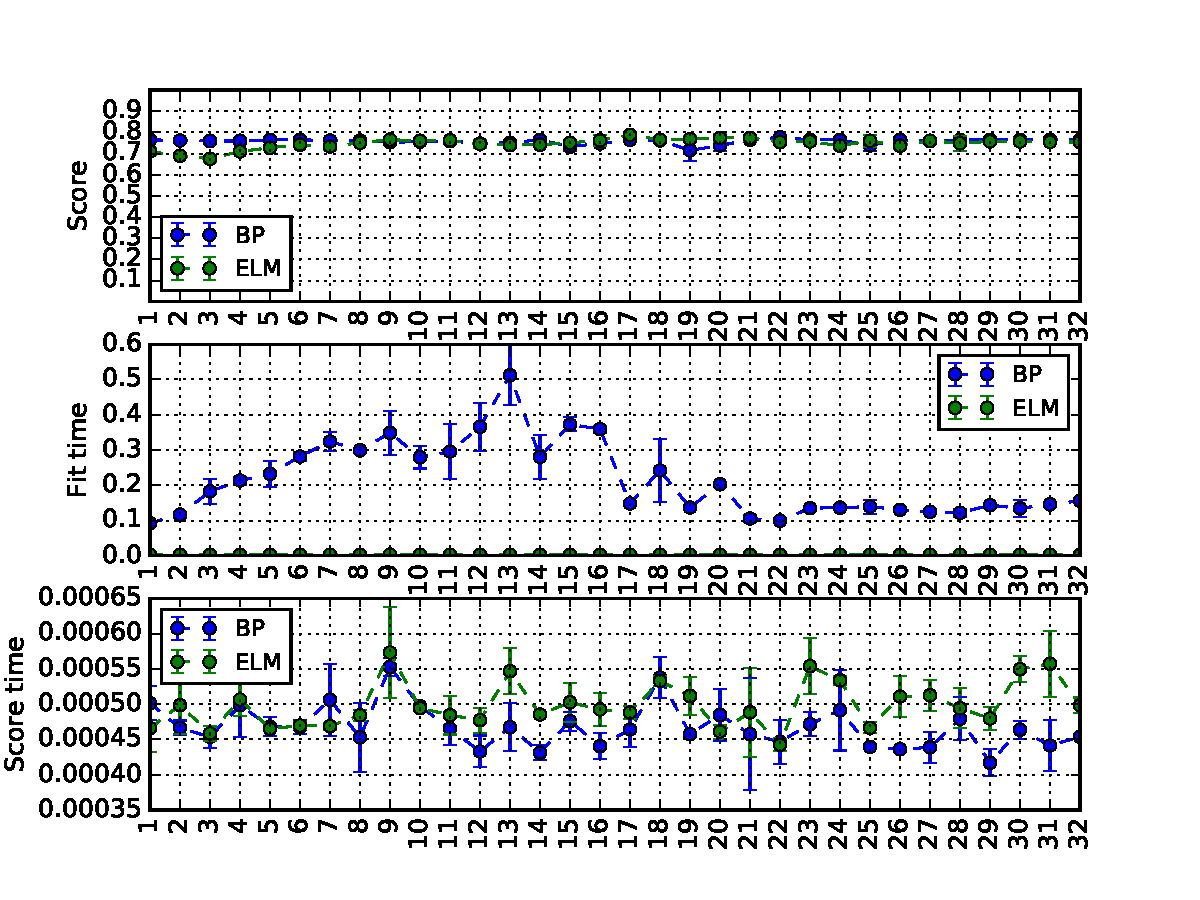
\includegraphics[width=1.0\linewidth]{img/bp_elm_20.pdf}
	\label{Rysunek}
	\caption{20 neuronów w warstwie ukrytej - porównanie obu algorytmów}
\end{figure}

\newpage

Dla 40 neuronów w warstwie ukrytej widać już bardzo wyraźnie zauważone wcześniej tendencje dla algorytmu \texttt{BP}. Reszta zależności pozostaje bez zmian.

\begin{figure}[h!]
	\centering
	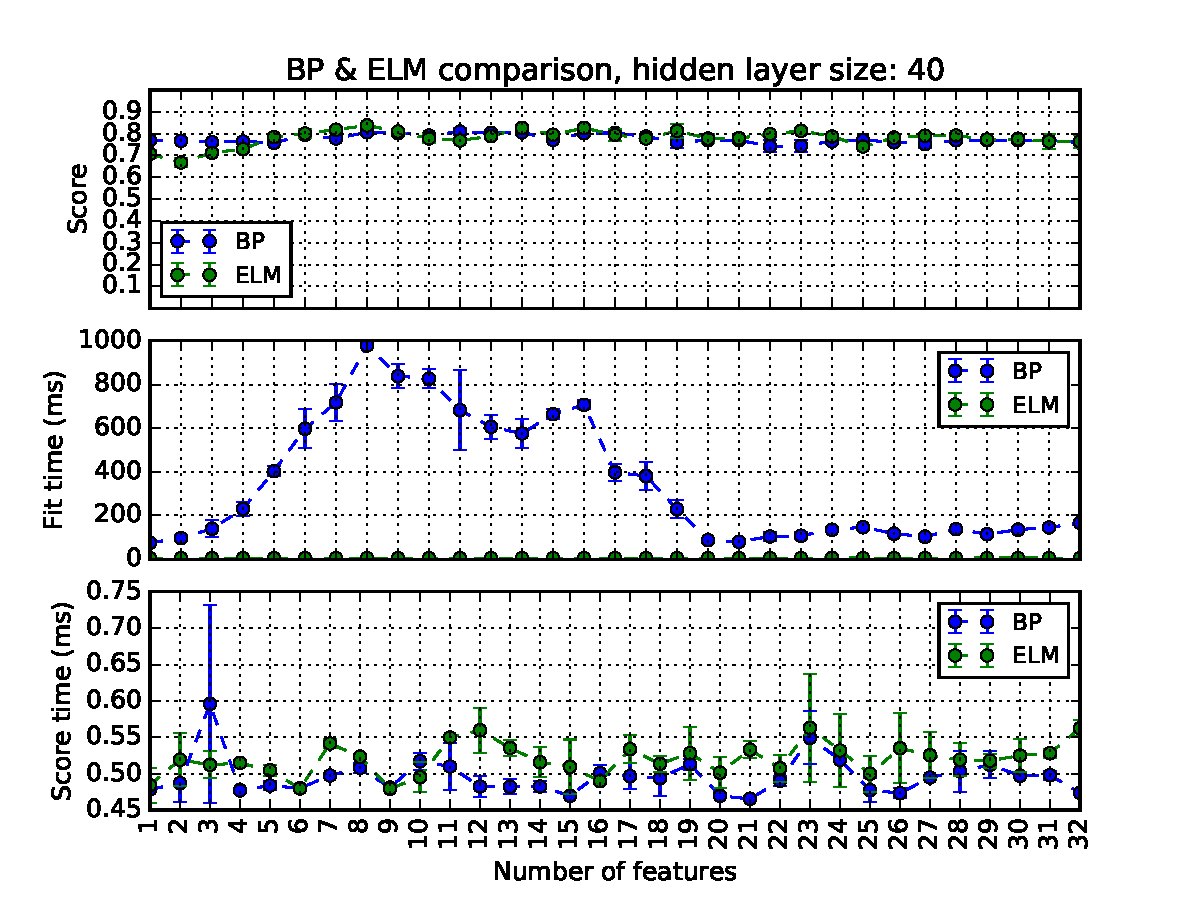
\includegraphics[width=1.0\linewidth]{img/bp_elm_40.pdf}
	\label{Rysunek}
	\caption{40 neuronów w warstwie ukrytej - porównanie obu algorytmów}
\end{figure}

\newpage

Dla 60 neuronów w warstwie ukrytej widać, że powyższe zależności pogłębiły się znacząco i czas uczenia algorytmu \texttt{BP} osiągał 1.2 sekundy. 

\begin{figure}[h!]
	\centering
	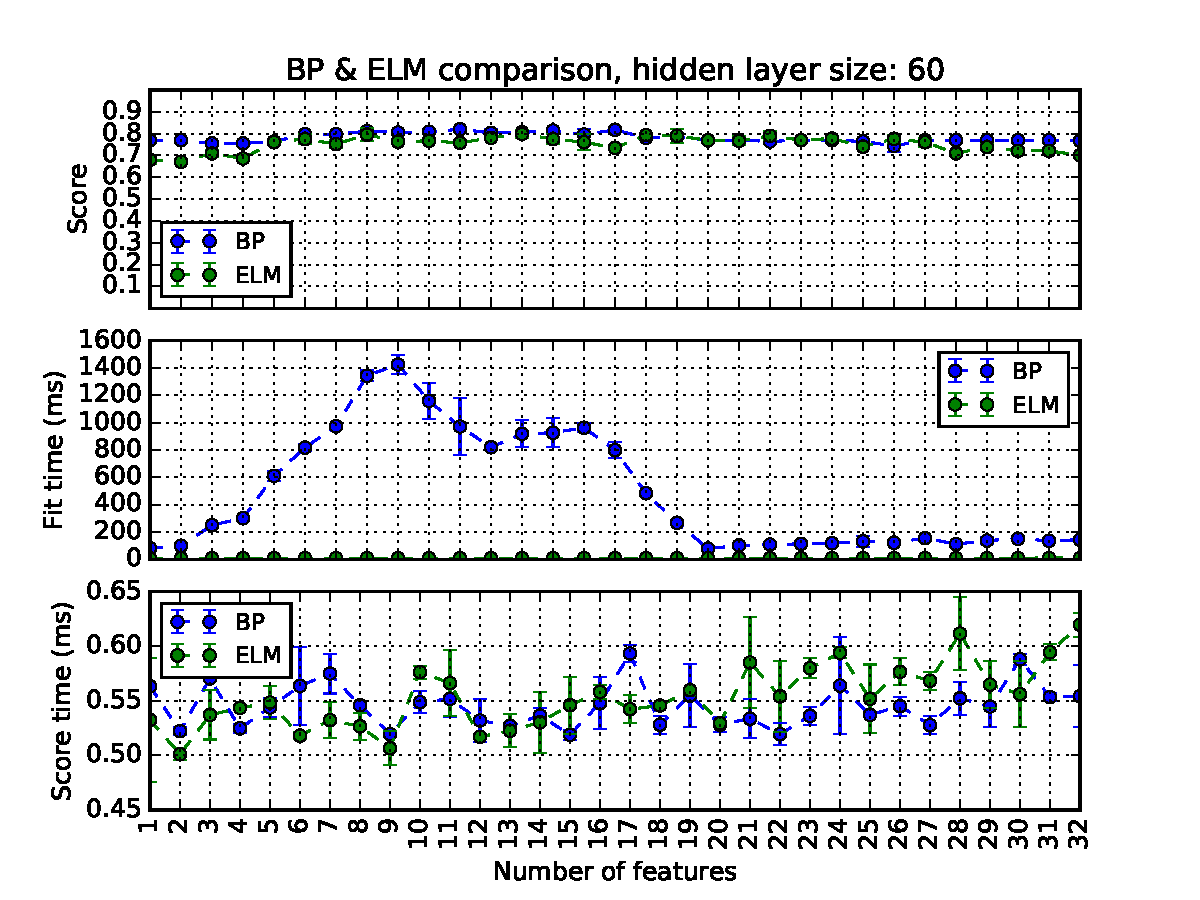
\includegraphics[width=1.0\linewidth]{img/bp_elm_60.pdf}
	\label{Rysunek}
	\caption{60 neuronów w warstwie ukrytej - porównanie obu algorytmów}
\end{figure}

\newpage

\section{Selekcja cech}
Selekcja cech polega na wybieraniu podzbioru cech w celu ograniczenia czasu uczenia, uproszczenia modelu oraz minimalizacji zjawiska przeuczenia.

W projekcie skorzystano z klasy \texttt{SelectKBest}, z modułu \texttt{sklearn.feature\_selection}.
\begin{figure}[h!]
	\centering
	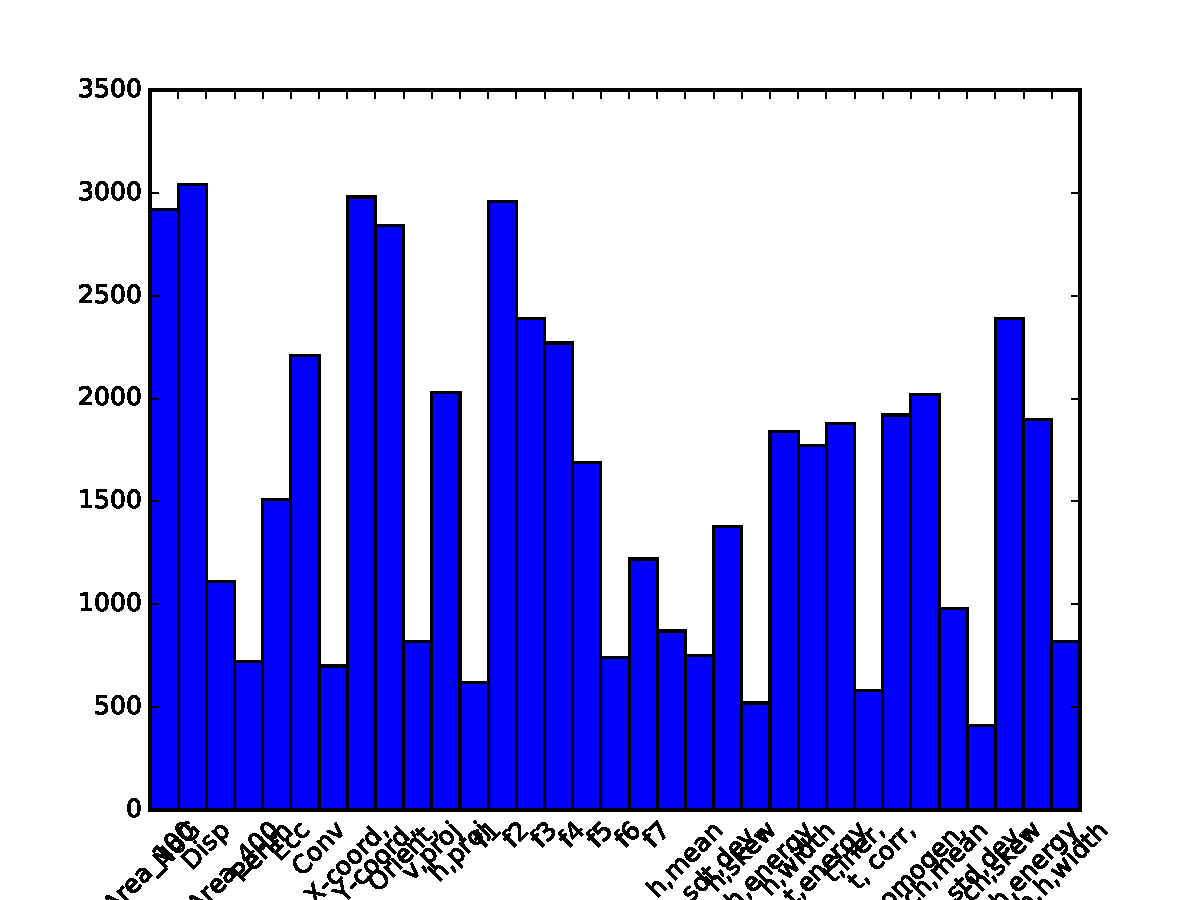
\includegraphics[width=1.0\linewidth]{img/features.pdf}
	\label{Rysunek}
	\caption{Częstość wybierania cech}
\end{figure}

\newpage

\section{Macierz pomyłek}
Macierz pomyłek umożliwia zobrazowanie jak dobrze klasyfikator radzi sobie ze swoim zadaniem.

Dla problemu z dwiema klasami -- tak jak w aktualnie rozpatrywanym problemie -- macierz dzieli się na cztery części, w których zliczane są obiekty sklasyfikowane poprawnie -- umieszczone na przekątnej macierzy -- oraz błędnie -- umieszczone poza przekątną.

W projekcie skorzystano z funkcji \texttt{confusion\_matrix}, z modułu \texttt{sklearn.metrics}.
\begin{figure}[h!]
	\centering
	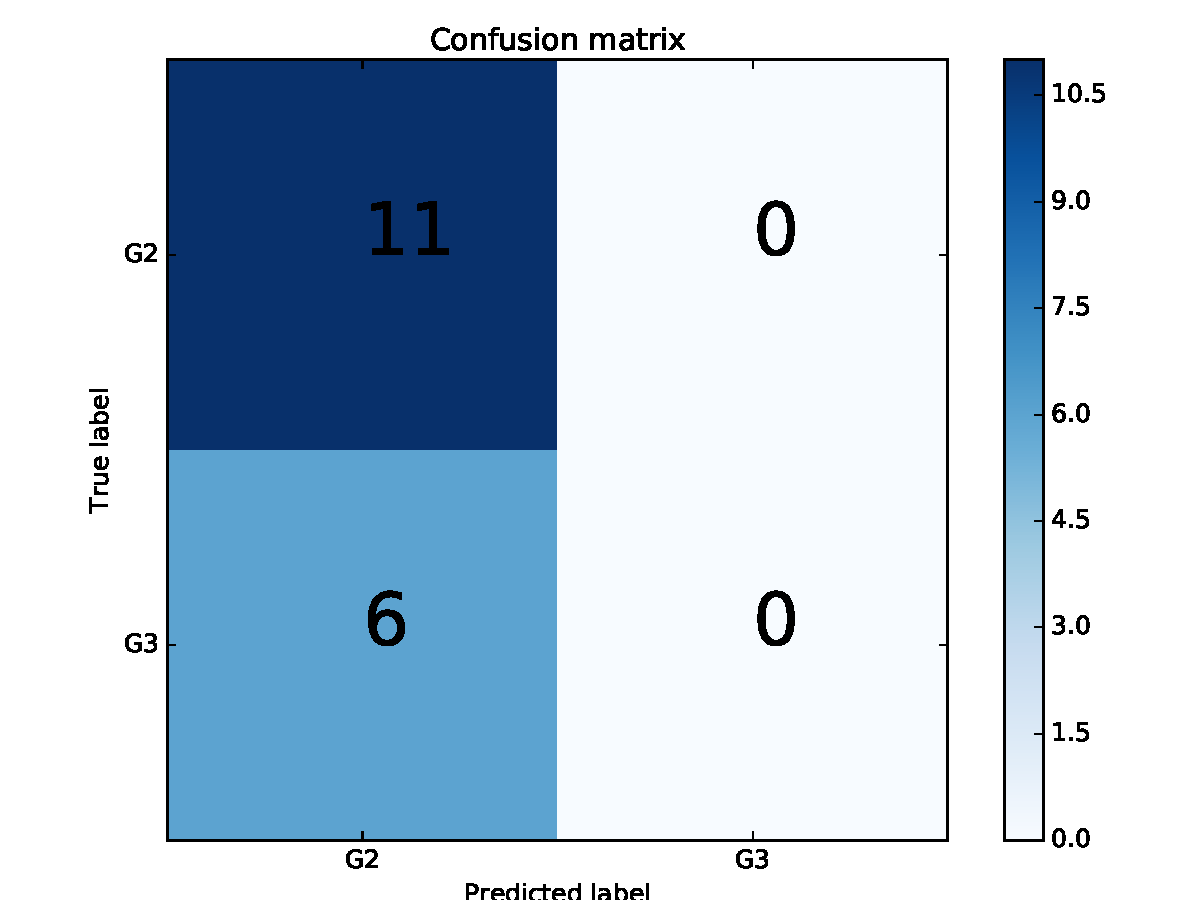
\includegraphics[width=1.0\linewidth]{img/conf_matrix.pdf}
	\label{Rysunek}
	\caption{Przykładowa macierz pomyłek}
\end{figure}
\chapter{Wnioski}
\begin{itemize}
	\item{Sieci neuronowe potrzebują sporej ilości danych uczących, aby poprawnie generalizować problemy.}
	\item{ELM daje bardzo zbliżone jakościowo wyniki do sieci neuronowych ze wsteczną propagacją, jednocześnie proces uczenia jest o wiele szybszy.}
	\item{Wbrew początkowej intuicji, kilka najlepszych cech zebranych razem wcale nie musi dawać najlepszych wyników.}
	\item{Procesy selekcji cech oraz walidacji krzyżowej nie mogą być przeprowadzane osobno.}
\end{itemize}

\end{document}
